\chapter{Estado del arte}


Para lograr atributos de calidad en el software, tales como modificabilidad, reusabilidad o mantenibilidad, es fundamental realizar un diseño del mismo basado en estilos arquitectónicos y patrones de diseño \cite{gamma,shawgarlan,buschmann}; es decir, aplicar las nociones centrales de la Ingeniería de Software.

Los sistemas de software para robots por lo general poseen alguna de las siguientes características: son distribuidos, embebidos, en tiempo real o manejan muchos datos. Su complejidad no termina ahí, deben encargarse del acceso al hardware, los algoritmos de navegación y decisión, entre otras responsabilidades, por lo tanto, muchas veces el diseño parece ser menos prioritario. Esto provoca que el esfuerzo se concentre en solucionar inconvenientes de implementación y no en diseñar cumpliendo los principios de la \textit{IS}.

En los trabajos que incluyen información relacionada al diseño \cite{bad-desing-auto,bad-desing-implantable,code-1,code-2,Zhang2009,bad-design-uml,bad-design-robot} encontramos que suele ser escasa y mostrarse como diagramas de flujo (ejemplo en \ref{flujo}), lo que deja en evidencia que el software esté implementado con un criterio de división funcional del código, con prácticas poco adecuadas (\textit{ifs} anidados (ejemplo en \ref{ifsanidados})) o con escasas funciones, es decir, con deficiencia de modularidad. Este tipo de división da como resultado que el código sea menos modificable, reusable y mantenible \cite{parnas72}. Por otro lado, como luego veremos, en algunos libros que intentan abordar este tema \cite{douglass} el resultado es similar.

\begin{figure}[h]
	\label{flujo}
    \centering
    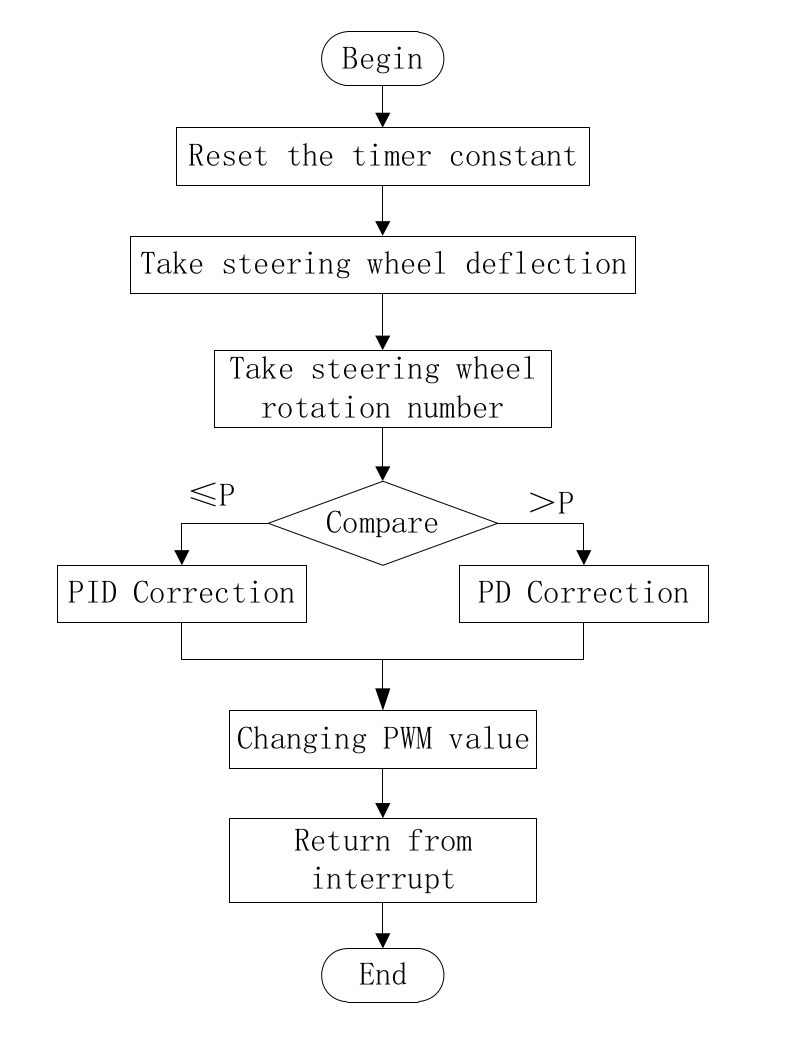
\includegraphics[width=0.5\linewidth]{diagrama_de_flujo.png}
    \caption{Diagrama de flujo que describe el comportamiento de parte de un sistema descripto en \cite{bad-desing-auto}}
\end{figure}

Hay ciertos trabajos \cite{good-desing-agrobot,good-desing-street} que tienen en cuenta algunos principios fundamentales de la \textit{IS} a la hora de diseñar y destinan esfuerzo en crear software de cierta calidad. Esto no significa que el uso de patrones de diseño esté generalizado.

Por otro lado, existen múltiples trabajos que abordan los ``patrones de diseño'' aplicados a un ámbito en particular. Por ejemplo, en \cite{enjambre} se proponen ``patrones'' con el formato de documentación de Gamma \cite{Gamma:1995:DPE:186897} que, según los autores, resultan útiles para diseñar sistemas de enjambres robóticos. Otro catálogo de patrones para una aplicación específica se encuentra en \cite{stable}, donde se describen patrones que ayudan a desarrollar sistemas robóticos estables, utilizando una definición particular de estabilidad. Asimismo, en la tesis \cite{critical} se proponen patrones orientados a lograr sistemas embebidos críticos seguros de manera efectiva, simple y rápida.

Podría pensarse entonces que existen múltiples trabajos que abordan patrones de diseño para sistemas embebidos de control o robóticos. Sin embargo, no es exactamente así. En los trabajos mencionados, se utiliza el concepto de patrón de diseño, pero no al nivel de diseño que se trabaja en la ingeniería de software. Los patrones presentados son más bien \textit{soluciones probadas para ciertos problemas recurrentes}. Es decir, los autores detallan cómo aplicar una solución a diversos inconvenientes comunes en sus áreas de estudio, pero no incluyen al diseño para el cambio a la hora de su confección. Además, en algunos de estos trabajos no se estudian módulos ni interfaces, sino componentes del sistema (algo más cercano a una arquitectura de software). De hecho, se llegan a documentar patrones para hardware, como ocurre con muchos de los patrones definidos en \cite{critical}.

La comunidad de Robótica ha comenzado a discutir sobre la necesidad de aplicar técnicas y principios de \textit{IS} para construir software robótico mantenible, reusable y modificable \cite{mejoras-1, mejoras-2}. E incluso se considera agregar formación relacionada a esta en cursos relacionados a robótica y sistemas embebidos \cite{Shin15fase}. Otra prueba del interés son desarrollos como \cite{FernandezMadrigal2003, model,model2,model3}, en los cuales se integran de diferentes maneras practicas de la \textit{IS} en el desarrollo de sistemas embebidos. Por un lado desarrollando \glspl{framework} y arquitecturas orientadas a este tipo de software, como también definiendo metodologías de trabajo. Estos \glspl{framework} no son los únicos orientados a este tipo de sistemas, existen por ejemplo \cite{framework-1, framework-ros}, los cuales son una mezcla de sistema operativo y framework. Estos representan fuertes herramientas para el desarrollo, principalmente, solucionan algunos inconvenientes recurrentes y le quitan responsabilidades al desarrollador resolviendo cuestiones relacionadas con el acceso al hardware, concurrencia, etc. Son ampliamente utilizados en la industria para grandes sistemas, ya que pueden resultar una solución demasiado pesada (dados sus requerimientos de hardware) o grande para algunos casos, como podrían ser ciertos sistemas de control.

Una de las principales motivaciones es la introducción de la robótica al mercado de consumo masivo fomentando la demanda de reducir los costos del software preservando sus cualidades. A medida que los sistemas embebidos incluyen más funciones para nuevos servicios, el software crece gradualmente en tamaño, y los costos y el tiempo de desarrollo también \cite{model2}. En particular, el diseño orientado al cambio, es una de las herramientas claves de la \textit{IS} para conseguirlo, ya que promueve la reusabilidad del software, haciéndolo aplicable a distintos proyectos y entornos. Esta es una muestra de que la implementación de patrones de diseño es una solución potencialmente útil y deseada.

